\chapter{Group Members}
\label{sec:groupmembers}
%\begin {table}[h]
    \begin{center}
    \begin{tabular}{|l|l|}\hline \rowcolor{white}
\multirow{7}{*}{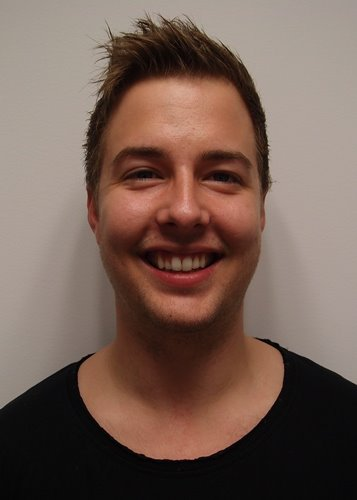
\includegraphics[width = 0.125\textwidth]{VAPIQ-PICTURES/tomas}} &  \textbf{Tomas Lyngroth}  \\
 &   \\
 & Phone: +47 45 09 95 88  \\
 & Mail: tomas.lyngroth@gmail.com  \\
 &   \\
 &  Mechanical Engineer \\
 &  Product Owner\\ \hline
 \multirow{7}{*}{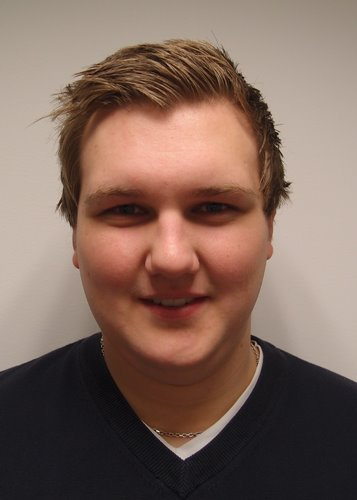
\includegraphics[width = 0.125\textwidth]{VAPIQ-PICTURES/stian}} & \textbf{Stian Fredriksen}  \\
 &   \\
 & Phone: +47 40 07 90 97  \\
 & Mail: stiann@live.no  \\
 &   \\
 & Software Engineer  \\
 & Scrum Master  \\ \hline
 \multirow{7}{*}{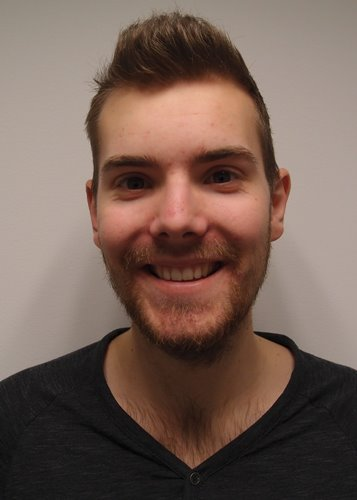
\includegraphics[width = 0.125\textwidth]{VAPIQ-PICTURES/kent}} & \textbf{Kent Kjeldaas}  \\
 &  \\
 & Phone: +47 41 22 98 33  \\
 & Mail: kent-kjeldaas@hotmail.com  \\
 &   \\
 & Software Engineer  \\
 & Lead Software Developer  \\ \hline
 \multirow{7}{*}{
\includegraphics[width = 0.125\textwidth]{VAPIQ-PICTURES/alex}} & \textbf{Aleksander Holthe}  \\
 &   \\
 & Phone: +47 94 22 50 79  \\
 & Mail: aleholthe@gmail.com  \\
 &   \\
 &  Signal Processing \\
 &  Interface \\ \hline
 \multirow{7}{*}{
\includegraphics[width = 0.125\textwidth]{VAPIQ-PICTURES/katrine}} & \textbf{Katrine Sundal Haune}  \\
 &   \\
 & Phone: +47 95 47 66 84  \\
 & Mail: katrinesundal@hotmail.com  \\
 &   \\
 & Cybernetics and Mechatronics  \\
 & Document Manager \\ \hline
 \multirow{7}{*}{
\includegraphics[width = 0.125\textwidth]{VAPIQ-PICTURES/vanja}} & \textbf{Vanja Katinka Halvorsen}  \\
 &   \\
 & Phone: +47 46 42 70 90  \\
 & Mail: vanja{\_}katinka@outlook.com  \\
 &   \\
 & Cybernetics and Mechatronics  \\
 & Test and Verification  \\ 
 \hline
    \end{tabular}
    \end{center}
%\end{table}
\newpage

\section{Responsibilities and Hierarchy}

A team contract has been formulated and agreed upon by all team members. The contract describes "codes of conduct", rules and norms within the group and guidelines on what to do when there is a breach in the contract. For more information see the group contract document in Appendix \textbf{\ref{app:groupcontract}}. The team has agreed upon a flat hierarchy structure. Each team member has the same amount of authority and all decision will be solved as democratically as possible, unless there is a disagreement. If there is a disagreement the product owner will have the final say.\bigskip

\textbf{Product Owner}\\
The Product Owner, also called Project Leader is responsible for: 
\begin{itemize}
  \item General supervision of the project
  \item Making sure the group is on schedule according to the short- and long-term plans
  \item Manage work efforts against the goal of the project without breaking the project boundaries 
  \item Report to supervisors about significant deviations from the project plan
  \item Ensuring good communication with internal and external supervisors
  \item Ensuring good communication within the group
\end{itemize}
\bigskip
\textbf{Scrum Master}\\
The Scrum Master is responsible for: 
\begin{itemize}
  \item Helping the team maintain their work velocity
  \item Setting up retrospectives, sprint reviews or sprint planning sessions
  \item Shielding the team from interruptions during the sprint
  \item Removing obstacles that affect the team
  \item Encouraging collaboration
\end{itemize}
\bigskip
\textbf{Interface manager}\\
The interface Manager is responsible for:
\begin{itemize}
  \item Responsible of cross disciplinary interfacing
  \item Ordering correct parts for the project
\end{itemize}
\bigskip
\textbf{Document Manager}\\
The Document Manager is responsible for:
\begin{itemize}
  \item See to that all documents are done
  \item See to that minutes of meetings are being written and distributed to the right people
  \item See to that all documents are proofread
  \item Document standards, ensure that all documents meets the chosen standard 
  \item See to that documents are signed by the right people
\end{itemize}
\newpage
\noindent\textbf{Test and Verification Manager}\\
The Test and Verification Manager is responsible for:
\begin{itemize}
  \item All test work relating to the group 
  \item Lead the work of testing
  \item Preparing the necessary test plans
\end{itemize}
\bigskip
\textbf{Mechanical Engineer}\\
The Mechanical Engineer is responsible for:
\begin{itemize}
  \item Managing the product design and construction
  \item Coordinating the documentation concerning mechanical design
\end{itemize}
\bigskip
\textbf{Software Engineer}\\
The Software Engineers are responsible for: 
\begin{itemize}
  \item Design flight controller
  \item Design program for autonomous flight 
  \item Coordinate documentation regarding software
\end{itemize}
\bigskip
\textbf{Electrical Engineer}\\
The Electrical Engineers are responsible for:
\begin{itemize}
  \item Electrical design and layout
  \item Control system for flight controller
  \item Coordinate documentation regarding control system and electronics
\end{itemize}

